\documentclass{standalone}
\usepackage{tikz}
\usetikzlibrary{patterns, positioning}

\begin{document}
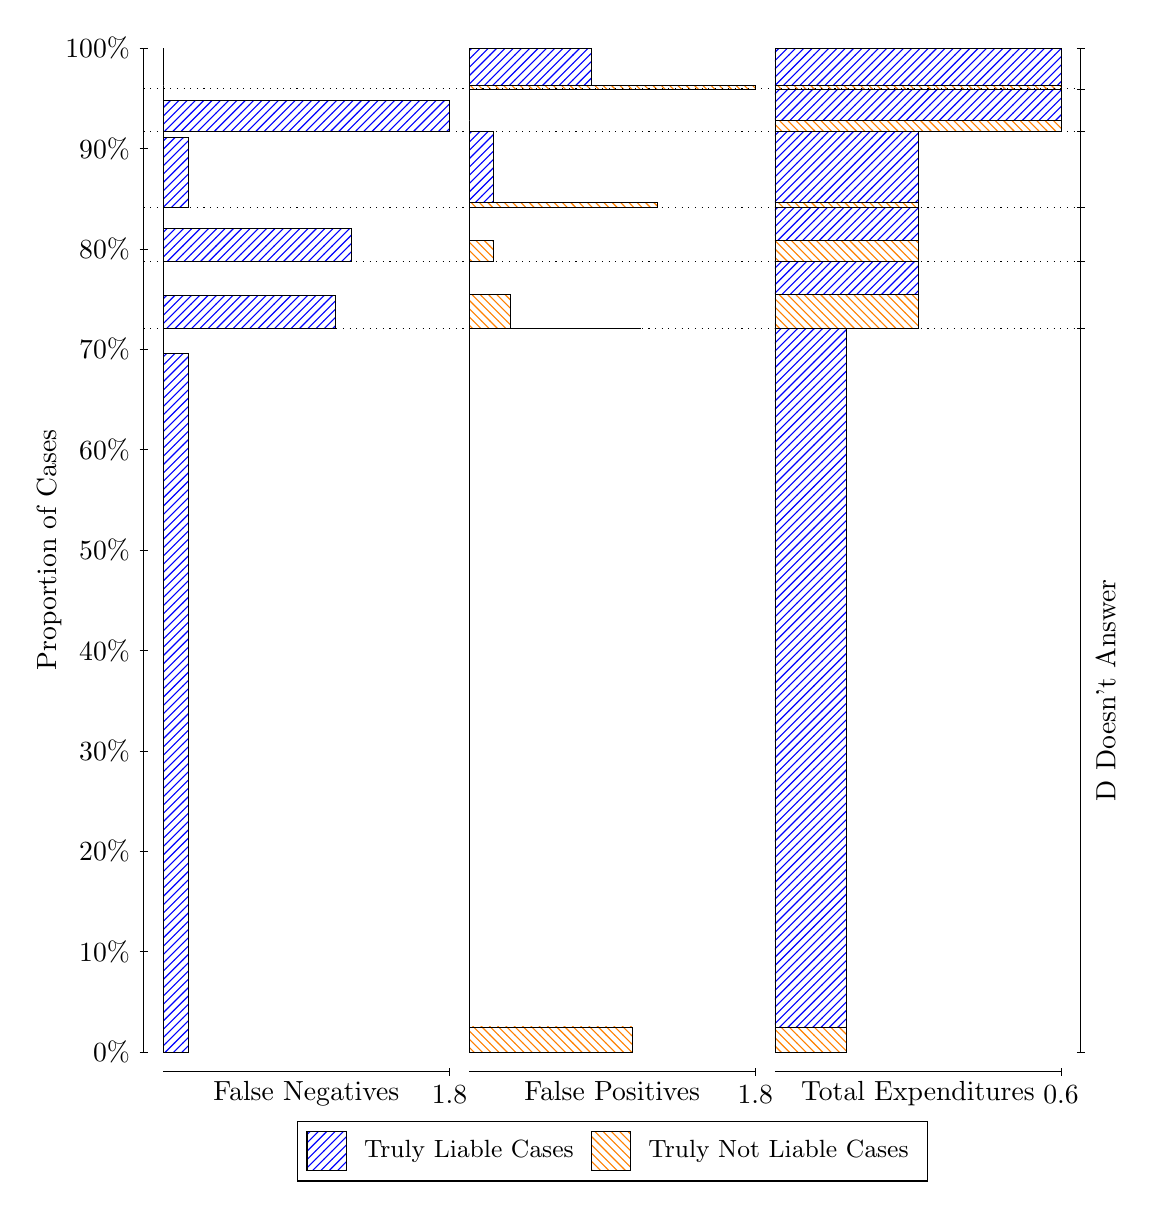
\begin{tikzpicture}
\draw[black, very thin] (1.5,1.75) -- (1.5,14.5);
\node[rotate=90, anchor=center] at (0.3, 8.125) {Proportion of Cases};
\draw[black, very thin] (1.45,1.75) -- (1.55,1.75);
\node[anchor=east] at (1.45, 1.75) {0\%};
\draw[black, very thin] (1.45,3.025) -- (1.55,3.025);
\node[anchor=east] at (1.45, 3.025) {10\%};
\draw[black, very thin] (1.45,4.3) -- (1.55,4.3);
\node[anchor=east] at (1.45, 4.3) {20\%};
\draw[black, very thin] (1.45,5.575) -- (1.55,5.575);
\node[anchor=east] at (1.45, 5.575) {30\%};
\draw[black, very thin] (1.45,6.85) -- (1.55,6.85);
\node[anchor=east] at (1.45, 6.85) {40\%};
\draw[black, very thin] (1.45,8.125) -- (1.55,8.125);
\node[anchor=east] at (1.45, 8.125) {50\%};
\draw[black, very thin] (1.45,9.4) -- (1.55,9.4);
\node[anchor=east] at (1.45, 9.4) {60\%};
\draw[black, very thin] (1.45,10.675) -- (1.55,10.675);
\node[anchor=east] at (1.45, 10.675) {70\%};
\draw[black, very thin] (1.45,11.95) -- (1.55,11.95);
\node[anchor=east] at (1.45, 11.95) {80\%};
\draw[black, very thin] (1.45,13.225) -- (1.55,13.225);
\node[anchor=east] at (1.45, 13.225) {90\%};
\draw[black, very thin] (1.45,14.5) -- (1.55,14.5);
\node[anchor=east] at (1.45, 14.5) {100\%};

\draw[black, very thin] (13.4,1.75) -- (13.4,14.5);
\draw[black, very thin] (13.35,1.75) -- (13.45,1.75);
\node[anchor=west] at (13.35, 1.75) {};
\draw[black, very thin] (13.35,10.939) -- (13.45,10.939);
\node[anchor=west] at (13.35, 10.939) {};
\draw[black, very thin] (13.35,11.79) -- (13.45,11.79);
\node[anchor=west] at (13.35, 11.79) {};
\draw[black, very thin] (13.35,12.474) -- (13.45,12.474);
\node[anchor=west] at (13.35, 12.474) {};
\draw[black, very thin] (13.35,13.437) -- (13.45,13.437);
\node[anchor=west] at (13.35, 13.437) {};
\draw[black, very thin] (13.35,13.981) -- (13.45,13.981);
\node[anchor=west] at (13.35, 13.981) {};
\draw[black, very thin] (13.35,14.5) -- (13.45,14.5);
\node[anchor=west] at (13.35, 14.5) {};

\draw[black, very thin, pattern color=blue, pattern=north east lines] (1.75,1.75) rectangle (2.0614,10.62);
\draw[black, very thin, pattern color=orange, pattern=north west lines] (1.75,10.62) rectangle (1.75,10.939);
\draw[black, very thin, pattern color=blue, pattern=north east lines] (1.75,10.939) rectangle (3.93,11.356);
\draw[black, very thin, pattern color=blue, pattern=north east lines] (1.75,11.356) rectangle (3.7224,11.356);
\draw[black, very thin, pattern color=blue, pattern=north east lines] (1.75,11.356) rectangle (3.5148,11.356);
\draw[black, very thin, pattern color=blue, pattern=north east lines] (1.75,11.356) rectangle (3.3071,11.356);
\draw[black, very thin, pattern color=blue, pattern=north east lines] (1.75,11.356) rectangle (3.0995,11.356);
\draw[black, very thin, pattern color=blue, pattern=north east lines] (1.75,11.356) rectangle (2.8919,11.356);
\draw[black, very thin, pattern color=blue, pattern=north east lines] (1.75,11.356) rectangle (2.6843,11.356);
\draw[black, very thin, pattern color=blue, pattern=north east lines] (1.75,11.356) rectangle (2.4767,11.356);
\draw[black, very thin, pattern color=blue, pattern=north east lines] (1.75,11.356) rectangle (2.269,11.356);
\draw[black, very thin, pattern color=orange, pattern=north west lines] (1.75,11.356) rectangle (1.75,11.79);
\draw[black, very thin, pattern color=blue, pattern=north east lines] (1.75,11.79) rectangle (4.1376,12.208);
\draw[black, very thin, pattern color=orange, pattern=north west lines] (1.75,12.208) rectangle (1.75,12.474);
\draw[black, very thin, pattern color=blue, pattern=north east lines] (1.75,12.474) rectangle (2.0614,13.37);
\draw[black, very thin, pattern color=orange, pattern=north west lines] (1.75,13.37) rectangle (1.75,13.437);
\draw[black, very thin, pattern color=blue, pattern=north east lines] (1.75,13.437) rectangle (5.3833,13.837);
\draw[black, very thin, pattern color=orange, pattern=north west lines] (1.75,13.837) rectangle (1.75,13.981);
\draw[black, very thin, pattern color=orange, pattern=north west lines] (1.75,13.981) rectangle (1.75,14.025);
\draw[black, very thin, pattern color=blue, pattern=north east lines] (1.75,14.025) rectangle (1.75,14.5);
\draw[black, very thin, pattern color=orange, pattern=north west lines] (5.6333,1.75) rectangle (7.7095,2.0693);
\draw[black, very thin, pattern color=blue, pattern=north east lines] (5.6333,2.0693) rectangle (5.6333,10.939);
\draw[black, very thin, pattern color=orange, pattern=north west lines] (5.6333,10.939) rectangle (7.8133,10.939);
\draw[black, very thin, pattern color=orange, pattern=north west lines] (5.6333,10.939) rectangle (7.6057,10.939);
\draw[black, very thin, pattern color=orange, pattern=north west lines] (5.6333,10.939) rectangle (7.3981,10.939);
\draw[black, very thin, pattern color=orange, pattern=north west lines] (5.6333,10.939) rectangle (7.1905,10.939);
\draw[black, very thin, pattern color=orange, pattern=north west lines] (5.6333,10.939) rectangle (6.9829,10.939);
\draw[black, very thin, pattern color=orange, pattern=north west lines] (5.6333,10.939) rectangle (6.7752,10.939);
\draw[black, very thin, pattern color=orange, pattern=north west lines] (5.6333,10.939) rectangle (6.7752,10.939);
\draw[black, very thin, pattern color=orange, pattern=north west lines] (5.6333,10.939) rectangle (6.5676,10.939);
\draw[black, very thin, pattern color=orange, pattern=north west lines] (5.6333,10.939) rectangle (6.36,10.939);
\draw[black, very thin, pattern color=orange, pattern=north west lines] (5.6333,10.939) rectangle (6.1524,11.374);
\draw[black, very thin, pattern color=blue, pattern=north east lines] (5.6333,11.374) rectangle (5.7371,11.374);
\draw[black, very thin, pattern color=blue, pattern=north east lines] (5.6333,11.374) rectangle (5.6333,11.79);
\draw[black, very thin, pattern color=orange, pattern=north west lines] (5.6333,11.79) rectangle (5.9448,12.056);
\draw[black, very thin, pattern color=blue, pattern=north east lines] (5.6333,12.056) rectangle (5.6333,12.474);
\draw[black, very thin, pattern color=orange, pattern=north west lines] (5.6333,12.474) rectangle (8.021,12.542);
\draw[black, very thin, pattern color=blue, pattern=north east lines] (5.6333,12.542) rectangle (5.9448,13.437);
\draw[black, very thin, pattern color=orange, pattern=north west lines] (5.6333,13.437) rectangle (5.6333,13.582);
\draw[black, very thin, pattern color=blue, pattern=north east lines] (5.6333,13.582) rectangle (5.6333,13.981);
\draw[black, very thin, pattern color=orange, pattern=north west lines] (5.6333,13.981) rectangle (9.2667,14.025);
\draw[black, very thin, pattern color=blue, pattern=north east lines] (5.6333,14.025) rectangle (7.1905,14.5);
\draw[black, very thin, pattern color=orange, pattern=north west lines] (9.5167,1.75) rectangle (10.425,2.0693);
\draw[black, very thin, pattern color=blue, pattern=north east lines] (9.5167,2.0693) rectangle (10.425,10.939);
\draw[black, very thin, pattern color=orange, pattern=north west lines] (9.5167,10.939) rectangle (11.333,10.939);
\draw[black, very thin, pattern color=blue, pattern=north east lines] (9.5167,10.939) rectangle (11.333,10.939);
\draw[black, very thin, pattern color=orange, pattern=north west lines] (9.5167,10.939) rectangle (11.333,11.374);
\draw[black, very thin, pattern color=blue, pattern=north east lines] (9.5167,11.374) rectangle (11.333,11.79);
\draw[black, very thin, pattern color=orange, pattern=north west lines] (9.5167,11.79) rectangle (11.333,11.79);
\draw[black, very thin, pattern color=blue, pattern=north east lines] (9.5167,11.79) rectangle (11.333,11.79);
\draw[black, very thin, pattern color=orange, pattern=north west lines] (9.5167,11.79) rectangle (11.333,12.056);
\draw[black, very thin, pattern color=blue, pattern=north east lines] (9.5167,12.056) rectangle (11.333,12.474);
\draw[black, very thin, pattern color=orange, pattern=north west lines] (9.5167,12.474) rectangle (11.333,12.542);
\draw[black, very thin, pattern color=blue, pattern=north east lines] (9.5167,12.542) rectangle (11.333,13.437);
\draw[black, very thin, pattern color=orange, pattern=north west lines] (9.5167,13.437) rectangle (13.15,13.582);
\draw[black, very thin, pattern color=blue, pattern=north east lines] (9.5167,13.582) rectangle (13.15,13.981);
\draw[black, very thin, pattern color=orange, pattern=north west lines] (9.5167,13.981) rectangle (13.15,14.025);
\draw[black, very thin, pattern color=blue, pattern=north east lines] (9.5167,14.025) rectangle (13.15,14.5);
\draw[black, dotted] (1.5,10.939) -- (13.4,10.939);
\draw[black, dotted] (1.5,11.79) -- (13.4,11.79);
\draw[black, dotted] (1.5,12.474) -- (13.4,12.474);
\draw[black, dotted] (1.5,13.437) -- (13.4,13.437);
\draw[black, dotted] (1.5,13.981) -- (13.4,13.981);
\draw[black, very thin] (1.75,1.5) -- (5.3833,1.5);
\node[anchor=north] at (3.5667, 1.5) {False Negatives};
\draw[black, very thin] (5.3833,1.45) -- (5.3833,1.55);
\node[anchor=north] at (5.3833, 1.45) {1.8};

\draw[black, very thin] (5.6333,1.5) -- (9.2667,1.5);
\node[anchor=north] at (7.45, 1.5) {False Positives};
\draw[black, very thin] (9.2667,1.45) -- (9.2667,1.55);
\node[anchor=north] at (9.2667, 1.45) {1.8};

\draw[black, very thin] (9.5167,1.5) -- (13.15,1.5);
\node[anchor=north] at (11.333, 1.5) {Total Expenditures};
\draw[black, very thin] (13.15,1.45) -- (13.15,1.55);
\node[anchor=north] at (13.15, 1.45) {0.6};

\node[black, centered, rotate=90] at (13.72, 6.3446) {D Doesn't Answer};






\draw (7.449999999999999,1.5) node[draw=none] (baseCoordinate) {};
\begin{scope}[align=center]
        \matrix[scale=0.5, draw=black, below=0.5cm of baseCoordinate, nodes={draw}, column sep=0.1cm]{
            \node[rectangle, draw, minimum width=0.5cm, minimum height=0.5cm, pattern=north east lines, pattern color=blue] {}; &
            \node[draw=none, font=\small] (B) {Truly Liable Cases}; &
            \node[rectangle, draw, minimum width=0.5cm, minimum height=0.5cm, pattern=north west lines, pattern color=orange] {}; &
            \node[draw=none, font=\small] (B) {Truly Not Liable Cases}; \\
            };
\end{scope}

\end{tikzpicture}
\end{document}